%%%%%%%%%%%%%%%%%%%%%%%%%%%%%%%%%%%%%%%%%
% kaobook
% LaTeX Template
% Version 1.2 (4/1/2020)
%
% This template originates from:
% https://www.LaTeXTemplates.com
%
% For the latest template development version and to make contributions:
% https://github.com/fmarotta/kaobook
%
% Authors:
% Federico Marotta (federicomarotta@mail.com)
% Based on the doctoral thesis of Ken Arroyo Ohori (https://3d.bk.tudelft.nl/ken/en)
% and on the Tufte-LaTeX class.
% Modified for LaTeX Templates by Vel (vel@latextemplates.com)
%
% License:
% CC0 1.0 Universal (see included MANIFEST.md file)
%
%%%%%%%%%%%%%%%%%%%%%%%%%%%%%%%%%%%%%%%%%

%----------------------------------------------------------------------------------------
%	PACKAGES AND OTHER DOCUMENT CONFIGURATIONS
%----------------------------------------------------------------------------------------

\documentclass[
	fontsize=11pt, % Base font size
	twoside=false, % Use different layouts for even and odd pages (in particular, if twoside=true, the margin column will be always on the outside)
	%open=any, % If twoside=true, uncomment this to force new chapters to start on any page, not only on right (odd) pages
	%chapterprefix=true, % Uncomment to use the word "Chapter" before chapter numbers everywhere they appear
	%chapterentrydots=true, % Uncomment to output dots from the chapter name to the page number in the table of contents
	numbers=noenddot, % Comment to output dots after chapter numbers; the most common values for this option are: enddot, noenddot and auto (see the KOMAScript documentation for an in-depth explanation)
	%draft=true, % If uncommented, rulers will be added in the header and footer
	%overfullrule=true, % If uncommented, overly long lines will be marked by a black box; useful for correcting spacing problems
]{kaobook}

% Set the language
\usepackage[english]{babel} % Load characters and hyphenation
\usepackage[english=british]{csquotes} % English quotes

% Load packages for testing
\usepackage{blindtext}
%\usepackage{showframe} % Uncomment to show boxes around the text area, margin, header and footer
%\usepackage{showlabels} % Uncomment to output the content of \label commands to the document where they are used

% Load the bibliography package
\usepackage{styles/kaobiblio}
\addbibresource{main.bib} % Bibliography file

% Load mathematical packages for theorems and related environments. NOTE: choose only one between 'mdftheorems' and 'plaintheorems'.
\usepackage{styles/mdftheorems}
%\usepackage{styles/plaintheorems}


\graphicspath{{images/}} % Paths in which to look for images

% \RequirePackage{times}

\DeclareMathOperator{\cA}{\mathcal A}
\DeclareMathOperator{\cB}{\mathcal B}
\DeclareMathOperator{\cC}{\mathcal C}
\DeclareMathOperator{\cD}{\mathcal D}
\DeclareMathOperator{\cE}{\mathcal E}
\DeclareMathOperator{\cF}{\mathcal F}
\DeclareMathOperator{\cG}{\mathcal G}
\DeclareMathOperator{\cM}{\mathcal M}
\DeclareMathOperator{\cN}{\mathcal N}
\DeclareMathOperator{\cP}{\mathcal P}

\DeclareMathOperator{\nor}{Normal}
\DeclareMathOperator{\ber}{Bernoulli}
\DeclareMathOperator{\bin}{Binomial}
\DeclareMathOperator{\mul}{Multinomial}
\DeclareMathOperator{\expo}{Exponential}
\DeclareMathOperator{\uni}{Uniform}

\DeclareMathOperator{\sigmoid}{sigmoid}

\newcommand{\eps}{\varepsilon}

\renewcommand{\P}{\mathbb P}
\newcommand{\E}{\mathbb E}
\newcommand{\R}{\mathbb R}
\newcommand{\var}{\mathbb V}

\newcommand{\wh}{\widehat}

\newcommand{\ind}[1]{\mathbf 1_{#1}}
\newcommand{\grad}{\nabla}


\newcommand{\mgeq}{\succcurlyeq}
\newcommand{\mleq}{\preccurlyeq}
\newcommand{\goes}{\rightarrow}
\newcommand{\go}{\rightarrow}

\newcommand{\norm}[1]{\|#1\|}

\newcommand{\gopro}{\overset{\P}{\rightarrow}}
\newcommand{\goas}{\overset{\text{as\ }}{\rightarrow}}
\newcommand{\gosto}{\leadsto}

\newcommand{\lest}{\underset{\text{st}}{\leq}}
\newcommand{\gest}{\underset{\text{st}}{\qeq}}



% \makeindex[columns=3, title=Alphabetical Index, intoc] % Make LaTeX produce the files required to compile the index

% \makeglossaries % Make LaTeX produce the files required to compile the glossary

% \makenomenclature % Make LaTeX produce the files required to compile the nomenclature

% Reset sidenote counter at chapters
%\counterwithin*{sidenote}{chapter}

%----------------------------------------------------------------------------------------

\begin{document}

%----------------------------------------------------------------------------------------
%	BOOK INFORMATION
%----------------------------------------------------------------------------------------

\titlehead{Some stuff about statistics}
\subject{Lecture notes for the ENS course of Statistics}

\title[Some stuff about Statistics]{Some stuff about Statistics}
% \subtitle{Customise this page according to your needs}

\author[St\'ephane Ga\"iffas"]{St\'ephane Ga\"iffas\thanks{}}

\date{\today}

\publishers{}

%----------------------------------------------------------------------------------------

\frontmatter % Denotes the start of the pre-document content, uses roman numerals

%----------------------------------------------------------------------------------------
%	OPENING PAGE
%----------------------------------------------------------------------------------------

%\makeatletter
%\extratitle{
%	% In the title page, the title is vspaced by 9.5\baselineskip
%	\vspace*{9\baselineskip}
%	\vspace*{\parskip}
%	\begin{center}
%		% In the title page, \huge is set after the komafont for title
%		\usekomafont{title}\huge\@title
%	\end{center}
%}
%\makeatother

%----------------------------------------------------------------------------------------
%	COPYRIGHT PAGE
%----------------------------------------------------------------------------------------

% \makeatletter
% \uppertitleback{\@titlehead} % Header

% \lowertitleback{
% 	\textbf{Disclaimer}\\
% 	You can edit this page to suit your needs. For instance, here we have a no copyright statement, a colophon and some other information. This page is based on the corresponding page of Ken Arroyo Ohori's thesis, with minimal changes.
	
% 	\medskip
	
% 	\textbf{No copyright}\\
% 	\cczero\ This book is released into the public domain using the CC0 code. To the extent possible under law, I waive all copyright and related or neighbouring rights to this work.
	
% 	To view a copy of the CC0 code, visit: \\\url{http://creativecommons.org/publicdomain/zero/1.0/}
	
% 	\medskip
	
% 	\textbf{Colophon} \\
% 	This document was typeset with the help of \href{https://sourceforge.net/projects/koma-script/}{\KOMAScript} and \href{https://www.latex-project.org/}{\LaTeX} using the \href{https://github.com/fmarotta/kaobook/}{kaobook} class.
	
% 	The source code of this book is available at:\\\url{https://github.com/fmarotta/kaobook}
	
% 	(You are welcome to contribute!)
	
% 	\medskip
	
% 	\textbf{Publisher} \\
% 	First printed in May 2019 by \@publishers
% }
% \makeatother

%----------------------------------------------------------------------------------------
%	DEDICATION
%----------------------------------------------------------------------------------------

% \dedication{
% 	The harmony of the world is made manifest in Form and Number, and the heart and soul and all the poetry of Natural Philosophy are embodied in the concept of mathematical beauty.\\
% 	\flushright -- D'Arcy Wentworth Thompson
% }

%----------------------------------------------------------------------------------------
%	OUTPUT TITLE PAGE AND PREVIOUS
%----------------------------------------------------------------------------------------

% Note that \maketitle outputs the pages before here

% If twoside=false, \uppertitleback and \lowertitleback are not printed
% To overcome this issue, we set twoside=semi just before printing the title pages, and set it back to false just after the title pages
\KOMAoptions{twoside=semi}
\maketitle
\KOMAoptions{twoside=false}

%----------------------------------------------------------------------------------------
%	PREFACE
%----------------------------------------------------------------------------------------

% \chapter*{Preface}
% \addcontentsline{toc}{chapter}{Preface} % Add the preface to the table of contents as a chapter

% I am of the opinion that every \LaTeX\xspace geek, at least once during 
% his life, feels the need to create his or her own class: this is what 
% happened to me and here is the result, which, however, should be seen as 
% a work still in progress. Actually, this class is not completely 
% original, but it is a blend of all the best ideas that I have found in a 
% number of guides, tutorials, blogs and tex.stackexchange.com posts. In 
% particular, the main ideas come from two sources:

% \begin{itemize}
% 	\item \href{https://3d.bk.tudelft.nl/ken/en/}{Ken Arroyo Ohori}'s 
% 	\href{https://3d.bk.tudelft.nl/ken/en/nl/ken/en/2016/04/17/a-1.5-column-layout-in-latex.html}{Doctoral 
% 	Thesis}, which served, with the author's permission, as a backbone 
% 	for the implementation of this class;
% 	\item The 
% 		\href{https://github.com/Tufte-LaTeX/tufte-latex}{Tufte-Latex 
% 			Class}, which was a model for the style.
% \end{itemize}

% The first chapter of this book is introductive and covers the most 
% essential features of the class. Next, there is a bunch of chapters 
% devoted to all the commands and environments that you may use in writing 
% a book; in particular, it will be explained how to add notes, figures 
% and tables, and references. The second part deals with the page layout 
% and design, as well as additional features like coloured boxes and 
% theorem environments.

% I started writing this class as an experiment, and as such it should be 
% regarded. Since it has always been indended for my personal use, it may 
% not be perfect but I find it quite satisfactory for the use I want to 
% make of it. I share this work in the hope that someone might find here 
% the inspiration for writing his or her own class.

% \begin{flushright}
% 	\textit{Federico Marotta}
% \end{flushright}


%----------------------------------------------------------------------------------------
%	TABLE OF CONTENTS & LIST OF FIGURES/TABLES
%----------------------------------------------------------------------------------------

% \begingroup % Local scope for the following commands

% % Define the style for the TOC, LOF, and LOT
% %\setstretch{1} % Uncomment to modify line spacing in the ToC
% %\hypersetup{linkcolor=blue} % Uncomment to set the colour of links in the ToC
% \setlength{\textheight}{23cm} % Manually adjust the height of the ToC pages

% % Turn on compatibility mode for the etoc package
% \etocstandarddisplaystyle % "toc display" as if etoc was not loaded
% \etocstandardlines % toc lines as if etoc was not loaded

% \tableofcontents % Output the table of contents

% \listoffigures % Output the list of figures

% % Comment both of the following lines to have the LOF and the LOT on different pages
% \let\cleardoublepage\bigskip
% \let\clearpage\bigskip

% \listoftables % Output the list of tables

% \endgroup

%----------------------------------------------------------------------------------------
%	MAIN BODY
%----------------------------------------------------------------------------------------

\mainmatter % Denotes the start of the main document content, resets page numbering and uses arabic numbers
\setchapterstyle{kao} % Choose the default chapter heading style


\setchapterpreamble[u]{\margintoc}
\chapter{Introduction}
\labch{intro}

\section{Aim of the course}

The aim of this course is, as the title indicated, to learn some stuff about statistics, and to try to exhibit some good looking mathematics from this field of applied mathematics, beyond convincing you that statistics are useful\sidenote{We won't list here, exhaustively, the numerous fields that make a regular use of mathematical statistics: marketing, medicine and more broadly health, finance, insurance, banking, etc.}

We will try to provide, all along the course, at material featuring 60\% of classical and unavoidable material from a course about statistics, and 40\% of more recent research results and some open questions.

The tentative agenda for the course is as follows:

\begin{itemize}
 	\item Modelization and the main statistical inference problems (estimation, confidence regions and tests)
 	\item Gaussian vectors and the Gaussian linear model
 	\item Theoretical guarantees and the optimality of least-squares
 	\item Estimation methods: methods of moments, maximum likelihood and other things
 	\item Exponential models and generalized linear models, logistic regression (optimal rates and some open questions)
 	\item Tests and multiple tests
 \end{itemize} 



\setchapterpreamble[u]{\margintoc}
\chapter{Statistical models}
\label{chap:statistical_models}

Let us start with the most classical and simplest statistical experiment: the coin toss.
We toss a coin $n$ times, and we model each toss by a random variable in $\{ 0, 1 \}$, where we decide that $1$ means that the toss ended up with heads (so that $0$ means tails).
To each toss is associated a random variable, leading to random variables $X_1, \ldots, X_n$  valued in $\{ 0, 1 \}$, where $X_i$ encodes the outcome of the $i$-th toss.
Each $X_i$ has distribution $\ber(p)$ for $p \in [0, 1]$, where $p$ corresponds to the probability that a coin toss gives heads, namely $\P(X_i = 1)$.%
\sidenote{The notation $\ber(p)$ corresponds to the \emph{Bernoulli distribution}: we will write $X \sim \ber(p)$ whenever $X \in \{ 0, 1\}$ and $\P(X = 1) = p = 1 - \P(X = 0)$.
Another way to obtain a $\ber$ distribution is by setting $X_i = \ind{Y_i \in A}$ where $Y_1, \ldots, Y_n$ are random variables valued in a probability space $(E, \cE)$, with $A \in \cE$, so that $X_i \sim \ber(p)$ with $p = \P(Y_i \in A)$.}
We assume that the $X_i$ are \emph{independent} (since the outcome of the tosses are physically unrelated), and since we are tossing the same coin each time, we assume that these outcomes have the same distribution (meaning that $p$ is constant along the tosses).
Therefore, we assume that $X_1, \ldots, X_n$ are \emph{iid}.%
\sidenote{From now on, iid will stand for \emph{independent and identically distributed}. More about this fundamental assumption will follow.}

\section{Probabilities and statistics} % (fold)
\label{sec:probability_versus_statistics}

Since we assume that the reader is familiar with the field of probabilities, we start this chapter with a comparison between what we do in probabilities and what we do in statistics for the $\ber(p)$ model described above.


\paragraph{Probabilities.} % (fold)

% paragraph probability (end)
In the field of probabilities, we suppose that $p \in (0, 1)$ is known, and we study the properties of the sequence $(X_i)_{i \geq 1}$. 
For instance, we know that the distribution of $S_n = \sum_{i=1}^n X_i$ is $\bin(n, p)$,  
namely that $\P(S_n = k) = \binom{n}{k} p^k (1 - p)^{n-k}$ for $k \in \{0, \ldots, n\}$.%
\sidenote{Where $\binom{n}{k}$ is the $(n, k)$ binomial coefficient given by $\frac{n!}{k! (n - k)!}$.}
It is easy to see that $\E(S_n) = n p$ and that $\var(S_n) = np (1 - p)$, where $\E(\cdot)$ and $\var(\cdot)$ stand respectively for the expectation and the variance.%
\sidenote{The linearity of the expectation gives $\E(S_n) = n \E(X_1) = np$ since the $X_i$ are identically $\ber(p)$ distributed, and, since the $X_i$ are iid, we know that $\var(S_n) = n \var(X_1) = n p (1 - p)$.}%
We can study the asymptotic properties of $S_n$, such as
\begin{equation}
	\label{eq:lln-binomial}
	\frac{S_n}{n} \goas p
\end{equation}
and
\begin{equation}
	\label{eq:tcl-binomial}
	\sqrt n \Big(\frac{S_n}{n} - p\Big) \leadsto \nor(0, p(1-p))
\end{equation}
as $n \rightarrow +\infty$, where $\nor(\mu, \sigma^2)$ stands for the Gaussian distribution with expectation $\mu$ and variance $\sigma^2$.%
\sidenote{The notation $X_n \goas X$ stands for the \emph{almost sure} convergence of $X_n$ towards $X$ while $X_n \leadsto X$ stands for the convergence of $X_n$ towards $X$ in distribution.}.
Note that statement~\eqref{eq:lln-binomial} comes from the law of large numbers, while~\eqref{eq:tcl-binomial} comes from the central limit theorem.
In the field of probabilities, the object of interest would be the \emph{random variable} $S_n$, that we study knowing the value of $p$.
In particular, if we replace the $\ber(p)$ distribution by the \emph{Rademacher distribution} $\text{Rademacher}(p)$ where $\P(X_i = 1) = 1 - \P(X_i = -1) = p$, the random variable $S_n$ becomes a \emph{random walk} for which many things can be said, depending on the value of $p$.%
\sidenote{But such things are way beyond the topic of this book, great references about the study of the random walk and its utmost importance in the field of probabilities are ???}

\paragraph{Statistics.} % (fold)

In statistics, for the $\ber(p)$ example, we don't really care about $S_n$, but we do care about $p$.
We assume that $p$ is \emph{unknown}, and we want to find out things about it.
This objective is called \emph{statistical inference} of the \emph{parameter} $p$.
For instance, we would like to know if $p=1/2$ or not, in order to find out if the coin is well-balanced and not rigged.
The random variables $X_1, \ldots, X_n$ (and $S_n$) live on some probability space $(\Omega, \cA, \P)$, but we don't really care about it either in statistics.
We will always assume, in statistics, that each \emph{observed} outcome $x_i \in \{ 0, 1 \}$ of a coin toss is a \emph{realization} of the random variable $X_i$, namely that
\begin{equation*}
	x_i = X_i(\omega)
\end{equation*}
for some \emph{event} $\omega \in \Omega$.
The realizations $x_i$ are also called \emph{data} or \emph{samples} or \emph{observations}.
But, actually, we will also refer to the random variables $X_i$ in the same way, as \emph{data}, \emph{samples} or \emph{observations}, since we won't manipulate the $x_i$ mathematically,%
\sidenote{nothing can be done with them... it's just deterministic zeros and ones}%
while we will work a lot with the random variables $X_1, \ldots, X_n$.
In statistics, we can do whatever we want with $X_1, \ldots, X_n$ in order to say things about $p$, but we will \emph{never} assume $p$ to be known.%
\sidenote{The parameter $p$ will quickly become a mathematical variable that we will use in equations, in order to perform calculus for instance. Therefore, we will use the specific notation $p_0$ for the ground truth parameter, namely $X_1 \sim \ber(p_0)$, while $p$ will be used as a generic parameter. A statistical parameter will usually be denoted as $\theta$, while the ground truth parameter will be denoted as $\theta_0$ when necessary.}
We will construct measurable functions of $(X_1, \ldots, X_n)$ that do not depend on $p$, these are called \emph{statistics}, in order to tell things about the unknown parameter $p$.
The object of interest in the field of statistics is, therefore, rather the \emph{distribution of the observations} than the observations themselves.


\section{Statistical models and experiences} % (fold)
\label{sec:statistical_models_and_experiences}

Let us consider another very classical problem: the election poll problem, where a population of size $N$ vote for one of two candidates $A$ and $B$.
There are $N_A$ people voting for $A$ while $N - N_A$ vote for $B$, and we want to know about $\theta_0 = N_A / N$.
We perform of poll including $n \ll N$ voters and obtain observations $x_1, \ldots, x_n \in \{ 0, 1 \}$, where $x_i = 0$ (resp. $x_i = 1$) means that voter $i$ votes for $B$ (resp. $A$).
In this problem, both $N_A$ and $N$ are so large that we can suppose that
\begin{equation*} 
	(x_1, \ldots, x_n) = (X_1(\omega), \ldots, X_n(\omega))
\end{equation*}
for some $\omega \in \Omega$, where all $X_i : (\Omega, \cA, \P) \rightarrow (\{0, 1\}, \cP(\{ 0, 1\})$ for $i=1, \ldots,, n$ are such that $X_i \sim \ber(\theta_0)$.
Let's look a little bit at all these mathematical objects. 
In statistics, we are mainly only interested by the fact that the observations are valued in $(\{0, 1\}, \cP(\{ 0, 1\})$ and that the distribution is $\P_{X_i} = \ber(\theta_0)$, which is fully described by its parameter $\theta_0 \in (0, 1)$.
Once again, we don't really care about $(\Omega, \cA, \P)$ in statistics.

\paragraph{Statistical model.}

The \emph{statistical model} for $X = (X_1, \ldots, X_n) \in \{0, 1\}^n$ is the family of distributions
\begin{equation*}
	\big\{ \P_\theta^{\otimes n} : \theta \in (0, 1) \big\}	= \big\{ \ber(\theta)^{\otimes n} : \theta \in (0, 1) \big\},
\end{equation*}
which is a family indexed by $\theta \in (0, 1)$.
The notation $\P^{\otimes n} = \P \otimes \cdots \otimes \P$ stands for the tensor product, namely $\P^{\otimes n}(A_1 \times \cdots \times A_n) = \prod_{i=1}^n \P(A_i)$ for any $A_i \in \cA$, $i=1, \ldots, n$.%
\sidenote{In this book, we will quickly forget to write $\P^{\otimes n}$ and we will write simply $\P$, when computations are clear enough, to avoid overloaded notations.}
When we say that this is a statistical model for $X$, we assume that there exist $\theta_0 \in (0, 1)$ such that $X \sim \ber(\theta_0)$.
Once again, let us insist on the following: we do whatever we want with $X_1, \ldots, X_n$ but never with $\theta_0$, which is the unknown parameter.

\paragraph{Another (naive) example.}

Let us consider the problem of the quality of production of screws. 
The dimensions of the screws must satisfy some strong constraints, for instance their length must match quite accurately some fixed size.%
\sidenote{The author of this book does not know anything about screws.}%
\begin{marginfigure}%
	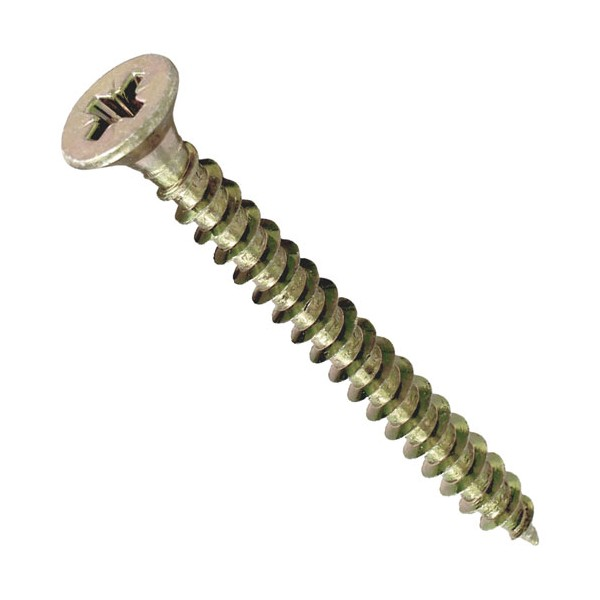
\includegraphics{screw.jpg}%
	\caption{I can't resist the idea of showing you a screw, so here it is.}%
\end{marginfigure}%
Millions of screws come out of the production chain, and we can't test all of them.
Therefore, we need to assess the production quality by selecting at random a small set of $n$ screws, and we measure their lengths $x_1, \ldots, x_n$.
Since these lengths are highly concentrated around the theoretical desired length $\mu$, and since production errors are usually small, we decide to choose a Gaussian model: we assume that $x_i = X_i(\omega)$ for $X_i \sim \nor(\mu, \sigma^2)$, where $\sigma^2$ corresponds to a small variance coming from the tiny production errors.

\emph{A model is a simplification of the reality.} For this example, we made the following modeling assumptions:

\textbf{ICI ICI ICI ICI ICI ICI}

\begin{description}
	\item[Distribution choice.] If we choose a $\nor(\mu, \sigma^2)$, then we implicitely assume that the true underlying distribution of the screws lengths is, among other things, symmetrical\sidenote{DEFINE SYMMETRICAL} and highly concentrated around $\mu$.
	\item[The i.i.d assumption.] Assuming that measurments are i.i.d means that weve been careful in the way we selected the screws produced (not the same days, not from the same producing machine, in order to avoid time and machine biases.)
\end{description}

A statistical model is \emph{always a simplification and an approximation of the truth}.
By truth we mean the true distribution $\P_{(X_1, \ldots, X_n})$ of $(X_1, \ldots, X_n)$.

Let us look at the $\nor(0, 1)$ distribution with density $\phi(x) = e^{-x^2/2} / \sqrt{2 \pi}$ supported on $\R$, while observations are usually bounded.
We can prove that if $Z \sim \nor(0, 1)$, then
\begin{equation*}
	\Big( \frac 1t - \frac{1}{t^3} \Big) \frac{1}{\sqrt{2\pi}} e^{-t^2 / 2} \leq \P(Z > t) \leq \frac{1}{t \sqrt{2 \pi}} e^{-t^2 / 2}
\end{equation*}
which means that the queues of the $\nor$ distribution are very tight.
For $t=6$ this entails that $\P(Z > t) \leq 10^{-9}$: we cannot distinguish between a variable supported in $[-6, 6]$ and a $\nor(0, 1)$.\todo{bof bof attention}

\begin{definition}
	A statistical experiment consists o
	\begin{itemize}
		\item A random object $X$ valued in a probability space $(E, \cE)$
		\item A family of distributions $\cP = \{ P_\theta : \theta \in \Theta\}$ on $(E, \cE)$.
	\end{itemize}
	We suppose that $\P_X = \P \circ X^{-1} \in \cP$. We say that $\cP$ is a \emph{statistical model} for $X$.
\end{definition}
The random variable $X : (\Omega, \cA, \P) \rightarrow (E, \cE)$ has distribution  $\P_X = \P \circ X^{-1}$ which is the probability image of $\P$ by $X$ on $(\Omega, \cA)$.

We will always suppose that there is a family $\{ \P_\theta : \theta \in \Theta\}$ on $(\Omega, \cA)$ that induce $\{ P_\theta : \theta \in \Theta\}$ on $(E, \cE)$ and we will use the notations
\begin{equation*}
	P_\theta(A) = \P_\theta(X \in A) = \P_\theta[ \{ \omega \in \Omega : X(\omega) \in A \}] \quad \forall A \in \cE.
\end{equation*}

Let us insist on the fact that $(\Omega, \cA, \P)$ is  purely mathematical build and has no interest in statistics.
We can alway assume that $X$ is the identity function and that $(\Omega, \cA) = (E, \cE)$, and let us recall the transfer formula
\begin{equation*}
	\int f(X(\omega)) \P_\theta(d \omega) = \int f(x) P_\theta(dx).
\end{equation*}
Because of this formula, we can always work only with $P_\theta$ and forget about $\P_\theta$ and the space $(\Omega, \cA)$.
We will often work with a space of parameters $\Theta \subset \R^d$, but this space can be much more complicated (such as infinite dimensional sets of functions with some smoothness properties, in this case we talk about nonparametric statistics.)

We will use the notation
\begin{equation*}
	\E_Q f(Y) := \int f(y) Q(dy)
\end{equation*}
where we implicitly assume, when computing this expectation, that $Y \sim Q$, and we wil shorten as following:
\begin{equation*}
	\E_\theta f(X) = \E_\theta f(X) = \int f(x) P_\theta(dx).
\end{equation*}
We will never work on $(\Omega, \cA, \P)$ but rather on $(E, \cE)$ and with the family $\cP$ (the statistical model).
\begin{definition}[Sampled experiment]
We have observations $X = (X_1, \ldots, X_n)$ with $X_i$ i.i.d and $\cP = \{ \P_\theta^{\otimes n} : \theta \in \Theta\}$, namely for $A = \prod_{i=1}^n A_i$ we have
\begin{align*}
	P_\theta^{\otimes n}(A) &= \P_\theta^{\otimes n}( (X_1, \ldots, X_n) \in A_1 \times \cdots A_n) = \prod_{i=1}^n \P_\theta(X_i \in A_i) \\
	&= \prod_{i=1}^n P_\theta(A_i).
\end{align*}
\end{definition}

Warning: we will quickly forget to distinguish between $\P_\theta$ and $P_\theta$ and $\P_\theta^{\otimes n}$ and $P_\theta^{\otimes n}$. 


Back to Bernoulli. We have $(E, \cE) = ({0, 1}^n, \cP(\{0, 1\}^n))$ and $P_\theta^{\otimes n} = \ber(\theta)^{\otimes n}$, $X = (X_1, \ldots, X_n)$ and $\Theta = (0, 1)$.
A ``roughly equivalent'' model is $S_n = \sum_{i=1}^n$ and $(E, \cE) = (\{ 0, \ldots, n\}, \cP(\{0, \ldots, n\}))$ with the same $\Theta = (0, 1)$.
Indeed, we have
\begin{equation*}
	\P_\theta^{\otimes n} (X_1 = x_1, \ldots, X_n = x_n | S_n=k) =
	\begin{cases}
	 & 0 \text{ if } k \neq \sum_{i=1}^n x_i \\
	 & \frac{\theta^k (1 - \theta)^{n-k}}{\binom{n}{k} 
	 \theta^k (1 - \theta)^{n-k}} = \frac{1}{\binom{n}{k} } \text{ otherwise.}
	\end{cases}
\end{equation*}
We observe that the conditional distribution of $(X_1, \ldots, X_n) | S$ \emph{does not depend} on $\theta$.
If we know $S$, then we can, without knowing $\theta$, build a sample $(X_1', \ldots, X_n')$ with the same distribution as $(X_1, \ldots, X_n)$, simply by choosing the $k$ among $n$ uniformly at random.
This means that $(X_1, \ldots, X_n)$ brings to more information about $\theta$ than $S_n$ alone.
In such a case, we say that $S_n$ is an \emph{exhaustive statistic}.

\begin{definition}
	Given a statistical experiment $X$, $\{ P_\theta : \theta \in \Theta \}$, we call \emph{statistic} any $X$-measurable function (a measurable function of $X$) which does not depend on $\theta$).
\end{definition}
\todo{doob lemma}
A statistic is therefore a quantity that we can compute using the data only.

\todo{Why $\theta_0$, we should say that there is a true parameter, well-specified model ?}

We want to say things about $\theta_0$ using $X$, but through $X$ we only have access to $\P_{\theta_0} = \P \circ X^{-1} = \P_X$.

\begin{definition}
	We say that a model $\cP = \{ P_\theta : \theta \in \Theta \}$ is \emph{identifiable} whenever the function
	\begin{align*}
		\Theta &\rightarrow \cP \\
		\theta &\mapsto P_\theta
	\end{align*}
	is injective.
\end{definition}


Identifiability is a necassary requirement when one want to perform statistical inference, namely whenever we can to find what the parameter $\theta$ is, only from data, namely realizations of $\P_\theta$.
If $\theta \mapsto \P_\theta$ is not injective, then there is no way to find back $\theta$ from $X \sim \P_\theta$.

Let us give simple examples: $\theta \mapsto \ber(\theta)$ is injective on $(0, 1)$ and $x \mapsto \ber(\sigmoid(x))$ is injective on $\R$.\sidenote{The sigmoid function is given by $\sigmoid(x) = \frac{1}{1 + e^{-x}}$. We will see later that this distribution function is of importance in statistics and machine learning.}

A stupid example of non-identifiable model is for instance $\mu \mapsto \nor(\mu^2, 1)$.
Identifiability is generally an interesting property, that you can ensure by choosing and parametrizing your model cleverly.
A more interesting example of non-identifiable model than the previous one is 
mixture models, such as the Gaussian mixture model where we consider a distribution with density
\begin{equation*}
	f_\theta(x) = \sum_{k=1}^K \pi_k \phi_{\mu_k, \Sigma_k}(x)
\end{equation*}
for any $x \in \R^d$, where $\theta = (\pi_k, \mu_k, \Sigma_k)_{k=1, \ldots, K}$ and $K \geq 1$ is an integer corresponding to the number of ``clusters'' in this mixture density.%
\sidenote{In the paramatrization of the Gaussian mixture we have $\mu_k \in \R^d$, $\Sigma_k \in \R^{d \times d}$ and $\Sigma_k \succ 0$ (meaning that $\Sigma_k$ is a symmetric positive matrix and $\pi_k \geq 0$ with $\sum_{k=1}^K \pi_k = 1$).}

A mixture density is not identifiable, since $f_{\theta} = f_{\sigma(\theta)}$
for any permutation $\sigma$ of $\{1, \ldots, K \}$, where we put $\sigma(\theta) = (\pi_{\sigma(k)}, \mu_{\sigma(k)}, \Sigma_{\sigma(k)})_{k=1, \ldots, K}$, namely we just relabel the numbering of the clusters.
Such mixture models are not identifiable, but are used often for clustering for instance (and instance of unsupervised learning, more on that later).
The situation is even worse for neural networks, in which an infinitely large number of parametrizations leads to the same cost function.

\section{Some types of models} % (fold)
\label{sec:some_types_of_models}

Whenever $\cP = \{ P_\theta : \theta \in \Theta \}$ with $\Theta \subset \R^d$ we say that $\cP$ is a \emph{parametric} model, since it is parametrized by a finite-dimensional parameter, trivial instances being $\{ \ber(\theta) : \theta \in (0, 1) \}$ for which $d=1$ and $\{ \nor(\mu, v) : (\mu, v) \in \R \times (0, +\infty) \}$ for which $d=2$.
We say that both models are \emph{dominated}, the first being dominated by the counting measure $\nu = \delta_0 + \delta_1$ on $\{ 0, 1\}$ and the second by the Lebesgue measure on $\R$.\sidenote{We recall that if $P$ and $Q$ are two measures on the same probability space, $P \ll Q$ means that the measure $P$ is \emph{absolutely continuous} with respect to $Q$, namely that $Q(A) = 0 \Rightarrow P(A)= 0$ for any measurable set $A$.}
\begin{definition}
	\label{def:dominated-model}
	We say that a model $\cP = \{ P_\theta : \theta \in \Theta \}$ is dominated if there is a $\sigma$-finite measure $\mu$ such that $P_\theta \ll \mu$ for all $\theta \in \Theta$.
\end{definition}
In Definition~\ref{def:dominated-model}, we require that the dominating measure is $\sigma$-finite, so that we can apply the Radon-Nikodym theorem: since $P_\theta \ll \mu$ for all $\theta \in \Theta$, then there is a density 
\begin{equation*}
	f_\theta = \frac{dP_\theta}{d\mu}
\end{equation*}
for all $\theta \in \Theta$.
The domination property allows to work with densities instead of distribution: a model can be therefore defined by a family of densities $\{ f_\theta : \theta \in \Theta \}$ together with a dominating measure (which is in most cases the Lebesgue measure, a counting measure, or a combination of them.)

Non-dominated models are usually pathological and uninteresting examples in statistics, such as the model
\begin{equation*}
	P_\lambda = \frac 1e \sum_{n \geq 0} \frac{1}{n!} \delta_{\lambda n}
\end{equation*}
for $\lambda \in (0, +\infty)$, which cannot be dominated by a $\sigma$-finite measure.

Let us finish this chapter with an example of non-parametric model: we observe $X_1, \ldots, X_n$ with a density $f \in F$ with respect to the Lebesgue measure, where $F$ is the set of probability densities on $[0, 1]^d$ that are $C^2$ and such that $\grad^2 f(x) \mleq L \mathbf I_d$.\todo{define identity and the fact that bold letters are for matrices only} This is the set of gradient-Lipschitz probability densities.
In this setting, we work with an infinite dimensional set of parameters $F$, and need to build a \emph{non-parametric} estimator of the unknown density $f$.


\setchapterpreamble[u]{\margintoc}
\chapter{Statistical inference}
\label{chap:statistical_inference}

In this Chapter, we will consider all along the most simple Bernoulli model, where we have i.i.d samples $X_1, \ldots, X_n$ distributed as $\ber(\theta)$ with $\theta \in (0, 1)$, hence the model $\cP = \{ \ber(\theta) : \theta \in (0, 1) \}$.
Let us start with the first inference problem: \emph{estimation}.
\todo{citer birge et son approche?}

\section{Estimation} % (fold)
\label{sec:estimation}

We want to infer $\theta$, or estimate it by finding a (measurable) function of $(X_1, \ldots, X_n)$\sidenote{Since we are doing statistics, the only thing we are allowed to use is the data...} or a function of $S_n = \sum_{i=1}^n X_i$ thereof, since $S_n$ is sufficient (see ??), so that there is no information loss if we look for a function of $S_n$ only, that we will denote
\begin{equation*}
 	\wh \theta_n = \wh \theta(X_1, \ldots, X_n).
\end{equation*}
Of course, this function \emph{cannot depend} on $\theta$, since once again, we are doing statistics.
Ideally, we want $\wh \theta_n$ to be "close" to $\theta$, since we want a good estimator, so we need to quantify closeness.
For instance, we could want $|\wh \theta_n - \theta|$ to be close to $0$ with a large probability, let us not forget that $\wh \theta_n$ is random, since it depends on the samples $(X_1, \ldots, X_n)$, so that quantifying the closeness of $\wh \theta_n$ to $\theta$ means controlling a stochastic quantity such as $|\wh \theta_n - \theta|$.
The most classical way to achieve this is by introducing the \emph{quadratic risk}.
\begin{definition}[Quadratic risk]
	Consider a statistical model with data $X$ and model with $\Theta \subset \R$ and an estimator $\wh \theta(X)$. The quadratic risk of $\wh \theta$ is given by
	\begin{equation*}
		R(\wh \theta, \theta) = \E_\theta[ (\wh \theta - \theta)^2 ] = \int_E (\wh \theta(x) - \theta)^2 P_\theta(dx).
	\end{equation*}
	We consider the quadratic risk as a function of the parameter, namely $\Theta \mapsto \R^+$ given by $\theta \mapsto R(\wh \theta, \theta)$.
\end{definition}
At this point, it's useful to recall some classical inequalities on the queues of random variables.
The Markov inequality tells us that if $Y$ is real random variable such that $\E |Y|^p < +\infty$ for some $p > 0$ then
\begin{equation*}
	\P(|Y| > t) \leq \frac{\E |Y|^p}{t^p}
\end{equation*}
for any $t > 0$.
This tells us that the more $Y$ has moments (an order $p$ moment means that $\E |Y|^p < +\infty$), with a large $p$, the more the queue of $Y$ is tight (it goes faster to $0$).
Markov's inequality entails easily the Bienaym\'e Tchebychev inequality
\begin{equation*}
	\P(|Y - \E Y| > t) \leq \frac{\var(Y)}{t^2}
\end{equation*}
whenever $\E Y^2 < +\infty$.
The Markov inequality entails, for $p=2$, that
\begin{equation}
	\label{eq:l2_entrails_proba}
	\P(|\wh \theta_n - \theta| > t) \leq \frac{R(\wh \theta, \theta)}{t^2}
\end{equation}
which entails that whenever the quadratic risk is small, then $\wh \theta$ is close to $\theta$ with a large probability.

Whenever $R(\wh \theta_n, \theta) \rightarrow 0$ with $n \rightarrow +\infty$, we say that $\wh \theta_n \rightarrow \theta$ in $L^2$\sidenote{More precisely, in $L^2(\P_\theta$}, which entails because of~\eqref{eq:l2_entrails_proba} that $\wh \theta_n \rightarrow \theta$ in probability.\sidenote{More precisely, in $\P_\theta$-probability. Let us recall at this point that $\wh \theta_n \rightarrow \theta$ in $\P_\theta$ probability whenever $\P_\theta[|\wh \theta_n - \theta| > \eps] \rightarrow 0$ as $n \rightarrow +\infty$ for any $\eps > 0$.}
When $\wh \theta_n \rightarrow \theta$ in probability, we say that $\wh \theta_n$ is a \emph{consistent} or \emph{convergent} estimator.
\begin{definition}
	We say that $\wh \theta_n$ is \emph{consistent} whenever $\P_\theta[|\wh \theta_n - \theta| > \eps] \rightarrow 0$ as $n \rightarrow +\infty$ for any $\eps > 0$ and any $\theta \in \Theta$.
	We say that it is strongly consistent whenever $\P_\theta[\wh \theta_n \rightarrow \theta] = 1$ and any $\theta \in \Theta$.
\end{definition}
In all these definitions, if $\Theta \subset \R^d$, it suffices to replace $|\cdot|$ by $\norm{\cdot}_2$ (or any other norm on $\R^d$)\sidenote{The norm $\norm{x}_2 = \sqrt{x^\top x} = (\sum_{j=1}^d x_j^2)^{1/2}$}


The bias-variance decomposition is the following decomposition of the quadratic risk between two terms: a bias term denoted $b(\wh \theta_n, \theta)$ (squared in the formula) and a variance term:
\begin{equation}
	\label{eq:bias-variance-decomposition}
	\begin{split}
	R(\wh \theta_n, \theta) &= \E_\theta[(\wh \theta_n - \theta)^2] = (\E_\theta \wh \theta_n - \theta)^2 + \var_\theta(\wh \theta_n) \\
	&= b(\wh \theta_n, \theta)^2 + \var_\theta(\wh \theta_n).		
	\end{split}
\end{equation}
When $b(\wh \theta_n, \theta) = 0$ for all $\theta \in \Theta$ we say that the estimator $\wh \theta_n$ is \emph{unbiased}.
This means that this estimator will not tend to over or under-estimate $\theta$. 

Going back to Bernoulli, we consider $\wh \theta_n = S_n / n = \sum_{i=1}^n X_i / n$, so that we have the following:
\begin{enumerate}
	\item We have $\E_\theta [\wh \theta_n] = \theta$ which means that $\wh \theta_n$ is unbiased;
	\item The bias-variance decomposition gives $R(\wh \theta_n, \theta) = \var(\wh \theta_n) = \theta (1 - \theta) / n \leq 1 / (4n) \rightarrow 0$ which means that $\wh \theta_n$ converges in $L^2$ (and that it is consistent) \todo{explain i.i.d variance etc.}
	\item The law of large number tells us that $\wh \theta_n \goes \theta$ almost surely.
	\item The central limit theorem tells us that $\sqrt n (\wh \theta_n - \theta) \leadsto \nor(0, \theta(1 - \theta))$.
\end{enumerate}
The points 2--4 from above show that when $n$ is large enough, then $\wh \theta_n$ is close to $\theta$.
In practice, an estimator leads to a value: for the Bernoulli model with $n=100$ and $42$ ones you end up with a single estimated value $0.42$.
What if we want to include uncertainty in this estimation ?
Namely how confident are we about this $0.42$ value ?
This can be achieved using another inference problem, described in the next section.

\section{Confidence intervals} % (fold)
\label{sec:confidence_intervals}

Here, we don't only want to build an estimator $\wh \theta_n$ but also to quantify the uncertainty of this estimation.
We saw in Equation~??? from Section~?? that 
\begin{equation*}
	\P_\theta[ |\wh \theta_n - \theta| > t] \leq \frac{1}{4 n t^2}
\end{equation*}
so that for $\alpha \in (0, 1)$ and the choice $t_\alpha = \frac{1}{2 \sqrt{n \alpha}}$ we have 
\begin{equation*}
	\P_\theta[ | \leq \theta \leq \wh \theta_n + \frac{1}{2 \sqrt{n \alpha}}| > t] \geq 1 - \alpha \text{ where } \wh \theta^L =  \wh \theta_n - \frac{1}{2 \sqrt{n \alpha}} \text{ and } \wh \theta^R =  \wh \theta_n + \frac{1}{2 \sqrt{n \alpha}} 
\end{equation*}
If we choose $\alpha = 0.05 = 5\%$, we know that $\theta \in [\wh \theta^L, \wh \theta^R]$ with a probability larger than $95\%$.
We say in this case that the interval $[\wh \theta^L, \wh \theta^R]$ is a \emph{confidence interval} with coverage $95\%$.

Note that if $\alpha = 0$ then we have no other choice than using $\R$ as a confidence interval, $\alpha$ allows to give some slack so that we can build a non-absurdly  large confidence interval. 
We typically have that $|\wh \theta^R - \wh \theta^L|$ increases as $\alpha$ decreases, since a smaller $\alpha$ means more confidence, hence a larger interval.
On the contrary, $|\wh \theta^R - \wh \theta^L|$ should decrease with the sample size $n$.
\begin{definition}[Confidence interval]
	Consider a statistical model with set of parameters $\Theta \subset \R$ and data $X$. Fix a \emph{confidence level} $\alpha \in (0, 1)$. 
	We say that $[\wh \theta^L(X), \wh \theta^R(X)]$ is a \emph{confidence interval} at level $1 - \alpha$ when $\wh \theta^L(X)$ and $\wh \theta^R(X)$ are statistics satisfying
	\begin{equation*}
		\P_\theta\{ \theta \in [\wh \theta^L(X), \wh \theta^R(X)] \} \geq 1 - \alpha
	\end{equation*}
	for any $\theta \in \Theta$.
\end{definition}
More generally when $\Theta \subset \R^d$ we will say that $D(X)$ is a \emph{confidence set} if it is a statistic satisfying $\P_\theta\{ \theta \in D(X) \} \geq 1 - \alpha$ for any $\theta \in \Theta$.

Remark. In some cases we can choose $\wh \theta^L = -\infty$ (or $0$ for the Bernoulli model) or $\wh \theta^R = +\infty$.
In this case we talk about a unilateral confidence interval.
This is interesting whenever we need to ensure that some toxicity level is smaller than some quantity.\sidenote{Using a unilateral IC allows to be slightly more precise on one side...}

But, we can do better for the Bernoulli model (or any model where $X$ is bounded) thanks to the Hoeffding inequality.
\begin{theorem}
	\label{thm:hoeffding}
	Let $X_1, \ldots, X_n$ be independent random variables such that $X_i \in [a_i, b_i]$ a.s. and let $S = \sum_{i=1}^n X_i$. Then, the following deviation inequality holds
	\begin{equation*}
		\P[ S \geq \E S + t] \leq \exp\Big( - \frac{2 t^2}{\sum_{i=1}^n (b_i - a_i)^2} \Big)
	\end{equation*}
	for any $t >0$.
\end{theorem}
Theorem~\ref{thm:hoeffding} is something called a deviation inequality: it provides a control on the probability of deviation of $S$ with respect to its mean.
This theorem shows that bounded random variables are \emph{sub-Gaussian}, since it shows that the queue of $S - \E S$ is bounded by $\exp(-c t^2)$ for some constant $c$ (although it depends on $n$).
\todo{Provide the proof of Hoeffding}

Let's apply Theorem~\ref{thm:hoeffding} to the Bernoulli case, where $X_i \sim \ber(\theta)$ so that $a_i = 0$, $b_i = 1$ and therefore $\P[ S \geq \E S + t] \leq e^{-2 t^2 / n}$.
By symmetry and the union bound\todo{side note Union bound} we have $\P[ | S - \E S | \geq t] \leq 2 e^{-2 t^2 / n}$ and for some $\alpha \in (0, 1)$ we obtain another confidence interval, since the following \emph{coverage property} holds:
\begin{equation*}
	\P \Big[ \theta - \sqrt{\frac{\log(2 / \alpha)}{2n}} \leq \theta \leq \wh \theta 
	+ \sqrt{\frac{\log(2 / \alpha)}{2n}} \Big] \geq 1 - \alpha.
\end{equation*}
This proves that the interval $[\wh \theta \pm \sqrt{\log(2 / \alpha) / (2n)}]$ is a confidence interval at level $1 - \alpha$.

Let's compare the two confidence intervals we obtained for the Bernoulli model.
We have of course
\begin{equation*}
	\frac{1}{2 \sqrt{n \alpha}} > \sqrt{\frac{\log(2 / \alpha)}{2n}} 
\end{equation*}
for $\alpha$ small enough, note also that both sides are $O(1 / \sqrt n)$.
Only the dependence on the level $\alpha$ is improved with the confidence interval obtained through the Hoeffding inequality, thanks to the sub-Gaussianity of the Bernoulli distribution, while we only used the second moment property for the first.
We just made a better use of the concentration properties of the Bernoulli distribution.
\sidenote{There is yet another way to build a (non-asymptotic) confidence interval, using a more computational approach, see for instance ????}

For both previous confidence intervals, we adopted a non-asymtotic approach: the coverage properties hold for any value of $n \geq 1$.
We were able to do this, since we able to use Hoeffding or since we know the exact distribution of $S_n$.

Let us now describe an asymptotic approach, which is the one typically used, since in general we don't know the exact distribution of the statistics used in the confidence intervals.
This approach is actually the one used in general, for more complicated models than Bernoulli, and is based on the central limit theorem.
Indeed, We know from the central limit theorem that
\begin{equation*}
	\sqrt{ \frac{n}{\theta(1 - \theta)}} (\wh \theta - \theta) =  \sqrt{\frac{n}{\var(X_1)}} \Big( \frac 1n \sum_{i=1}^n X_i - \E X_1 \Big) \leadsto \nor(0, 1)
\end{equation*}
which entails, for any interval $I \subset \R$\todo{borelien je sais pas quoi} that
\begin{equation*}
	\P_\theta\Big[ \sqrt n \frac{\wh \theta - \theta}{\sqrt{\theta(1 - \theta)}} 
	\Big] \rightarrow \P[Z \in I]
\end{equation*}
where $Z \sim \nor(0, 1)$.
Using $I = [-q_\alpha, q_\alpha]$ with $q_\alpha = \Phi^{-1}(1 - \alpha / 2)$ we end up with the fact that
\begin{equation*}
	\P_\theta\Big\{ \theta \in \Big[ \wh \theta \pm \frac{q_\alpha \sqrt{\theta(1 - \theta)}}{\sqrt n} \Big] \rightarrow 1 - \alpha.
\end{equation*}
All that is interesting enough, but useless, since the interval we built in Equation~??? depends on $\theta$ ! It is \emph{not} a confidence interval, we can't use it since it depends on $\theta$.
We need to work a little bit more in order to remove the dependence on $\theta$ from this interval. 
We can proceed as follows: we can use that $\theta (1 - \theta) \leq 1 / 4$ for any $\theta \in [0, 1]$, so that
\begin{equation*}
	\liminf_n \P_\theta\{ \theta \in [\wh \theta \pm \frac{q_\alpha}{2 \sqrt n} ] \} = 1 - \alpha.
\end{equation*}
This is what we call a confidence interval of \emph{asymptotically of level} $1 - \alpha$, constructed \emph{by excess}.

A problem with this approach is that we used the fact that the Binomial distribution (the distribution of $S_n$) correctly renormalized is approximated by a Gaussian distribution for large $n$.
This requires $n$ to be large enough, but also $\theta$ to be not to close to $0$ and $1$.
We quantify this better by looking at the closeness to the Gaussian distribution, using the following theorem.
\begin{theorem}[Berry Essen, see ????]
	Let $X_1, \ldots, X_n$ be i.i.d random variables such that $\E X_i = 0$ and $\var X_i = \sigma^2$ and introduce the distribution function
	\begin{equation*}
		F(x) = \P \Big[ \frac{\sum_{i=1}^n X_i}{\sqrt{n \sigma^2}} \leq x \Big]
	\end{equation*}
	for any $x \in \R$. Then, the following inequality holds:
	\begin{equation*}
		|F(x) - \Phi(x)| \leq \frac{3 \kappa}{\sigma^3 \sqrt n}
	\end{equation*}
	where $\kappa = \E |X_1|^3$ (implicitly assumed finite, otherwise the bound is trivial).
\end{theorem}
\todo{insert reference and proof ?}

For Bernoulli with have $\E|X_1|^3 = \theta$ and $\sigma^3 = (\theta(1 - \theta))^{3/2}$so that 
\begin{equation*}
	|F(x) - \Phi(x)| \leq \frac{3}{\sqrt{n \theta (1 - \theta)^3}}
\end{equation*}
which shows that the approximation by the Gaussian distribution deteriorates whenever $\theta$ is close to $0$ or $1$.


\todo{subsection ?}

Another approach to get rid of the dependence on $\theta$ from ??? is to use another asymptotic approach, based on reparametrization.
Indeed, given a statistical model $\{ P_\theta : \theta \in \Theta \}$ and a bijective function $g : \Theta \goes \Lambda$ we can use instead the "reparametrized" model $\{ Q_\lambda : \lambda \in \Lambda \}$ where $Q_\lambda = P_{g^{-1}(\lambda)}$.
Let us also remark that if $[\wh \theta^L, \wh \theta^R]$ is a confidence interval for $\theta$ at level $1 - \alpha$ and if $g$ is an increasing function, then 
$[g(\wh \theta^L), g(\wh \theta^R]$ is a confidence interval for $g(\theta)$ at level $1 - \alpha$.
Now, a natural question is to understand if the convergences we used above (in particular, convergence in distribution) is stable under such a reparametrization.

Example. If $X_1, \ldots, X_n$ is a i.i.d sample with distribution $\expo(\theta)$ with scale parameter $\theta > 0$, namely if $P_\theta(dx) = \theta e^{-\theta x} \ind{x \geq 0} dx$ we have $\E(X_1) = 1 / \theta$ and $\var(X_1) = 1 / \theta^2$, so that using the law of large numbers and the central limit theorem we have
\begin{equation*}
	\bar X_n \rightarrow \theta^{-1} \text{ a.s.  and } \sqrt (\bar X_n - \theta^{-1}) \leadsto \nor(0, \theta^{-2})
\end{equation*}
when $n \rightarrow +\infty$.
Since $x \mapsto 1 / x$ is a continuous function on $(0, +\infty)$, we know that $(\bar X_n)^{-1} \goes \theta$ a.s. so that we want to use the estimator $\wh \theta = (\bar X_n)^{-1}$.
But what can we say about the convergence in distribution of $\sqrt n (\wh \theta - \theta)$ ?
This is answered by the following $\Delta$-method
\begin{theorem}[$\Delta$-method]
	\label{thm:delta-method}
 	Let $(Z_n)_{n \geq 1}$ be a sequence of random variables in $\R$ and a sequence $(a_n)_{n \geq 1}$ such that $a_n > 0$ and $a_n \goes +\infty$ such that $a_n(Z_n - z) \leadsto Z$ for some $z \in \R$ and random variable $Z$.
 	If $g$ is a function defined on a neighborhood of $z$ and differentiable at $z$, we have 
 	\begin{equation}
 		a_n (g(Z_n) - g(z)) \leadsto g'(z) Z
 	\end{equation}
 	as $n \goes +\infty$.
\end{theorem}
The proof easily follows by a first-order Taylor expansion of $g$ around $z$.
\todo{insert proof}

A particularly useful special case for statistics is when $Z$ is Gaussian, for instance if we have $\sqrt n (\wh \theta - \theta) \leadsto \nor(0, \sigma(\theta)^2)$, when we have because of the $\Delta$-method
\begin{equation*}
	\sqrt n (g(\wh \theta) - g(\theta)) \leadsto 
	\nor(0, \sigma(\theta)^2 (g'(\theta))^2),
\end{equation*}
whenever $g$ satisfies the conditions of Theorem~\ref{thm:delta-method}.
Going back to the $\expo$ example, we obtain with $g(x) = 1 / x$ and since $\wh \theta = g(\bar X_n)$ that $\sqrt n (\wh \theta - \theta) \leadsto \nor(0, \theta^2)$.

Another result of the same nature is the so-called Slutsky theorem.
\begin{theorem}[Slutsky]
	Let $(X_n)_{n \geq 1}$ and $(Y_n)_{n \geq 1}$ be sequences of real random variables such that $X_n \leadsto X$ and $Y_n \leadsto y$ where $X$ is some real random variable and $y \in \R$ is a real number.
	Then, we have that $Y_n \goes y$ in probability and $(X_n, Y_n) \leadsto (X, y)$ as $n \goes +\infty$. In particular, we have $f(X_n, Y_n) \leadsto f(X, y)$ for any continuous function $f$.
\end{theorem}
\todo{insert proof}

Let's apply this to the Bernoulli case. 
We have that $\wh \theta \gopro \theta$, so that $\sqrt{\wh \theta (1 - \wh \theta)} \gopro \sqrt{ \theta (1 -  \theta)}$ since $\sqrt{x(1-x)}$ is continuous on $[0, 1]$ and 
therefore
\begin{equation*}
	\frac{\sqrt n (\wh \theta - \theta)}{\sqrt{\wh \theta (1 - \wh \theta)}} 
	= \frac{\sqrt n (\wh \theta - \theta)}{\sqrt{ \theta (1 -  \theta)}} \frac{\sqrt{ \theta (1 -  \theta)}}{\sqrt{\wh \theta (1 - \wh \theta)}} = A \times B.
\end{equation*}
We know from above that $A \gosto \nor(0, 1)$ and that $B \gopro 1$.
Therefore, using Slutsky's lemma\sidenote{With $f(x, y) = x y$} we have that
\begin{equation*}
	\frac{\sqrt n (\wh \theta - \theta)}{\sqrt{\wh \theta (1 - \wh \theta)}} \gosto \nor(0, 1).
\end{equation*}
This is somewhat pendantic for such an intuitive result, but this requires the Slutsky's theorem for a rigorous proof.

The $\Delta$-method provides stability for the convergence in distrubition when a locally differentiable function is applied to the sequence, while Slutky's theorem provides "algebraic" statibility when combining two sequences converging in distribution and probability.
\sidenote{Be careful with convergence in distribution. Please keep in mind that this convergence mode has nothing to do with random variables, but only with their distributions, hence its name. In particular, nothing can be said in general about $f(X_n, Y_n)$ when $X_n \gosto X$ and $Y_n \gosto Y$, a counter example being, among billions of others}
\todo{insert counter example here}

The last convergence leads to a last convergence interval asymptotically of level $1 - \alpha$, since we know now that
\begin{equation*}
	\P_\theta \bigg\{ \theta \in \Big[ \wh \theta \pm q_\alpha \sqrt{\frac{\wh \theta (1 - \wh \theta)}{n}} \Big] \bigg\} \goes 1 - \alpha
\end{equation*}
as $n \goes +\infty$.

\todo{some exercices ?}

\section{Tests} % (fold)
\label{sec:tests}

Let us consider in this section, once again a model $\{ P_\theta : \theta \in \Theta \}$ and a sample $X$.
Here, we want to decide between to hypothesis $H_0$ and $H_1$, where
\begin{equation*}
	H_i \text{ corresponds to the fact that } \theta \in \Theta_i
\end{equation*}
for $i \in \{ 0, 1 \}$, where $\{ \Theta_0, \Theta_1 \}$ is a partition of $\Theta$.

Let us give, to help understand this complex concept of statistical testing, a morbid example.
Imagine that you need to decide if a patient has cancer or not.
The patient has cancer if some parameter $\theta \in (0, 1)$ about him satisfies 
$\theta \geq 0.42$.
We \emph{choose} $\Theta_0 = [0.42, 1]$ and $\Theta_1 = [0, 0.42)$.
We need to construct a testing function $\varphi : E \goes \{ 0, 1 \}$ that maps $X \mapsto \phi(X)$, our decision being the value of $\varphi(X)$.
We are correct if $\varphi(X) = i$ whenever $\theta \in \Theta_i$ for $i \in \{ 0, 1 \}$ and incorrect whenever  $\varphi(X) = 1 - i$ whenever $\theta \in \Theta_i$.
We have two types of errors: the \emph{Type-I error} or \emph{first-order error}, given by 
\begin{equation}
	\label{eq:type-1-error}
	\P_\theta[ \varphi(X) = 1] = \E_\theta \varphi(X) \text{ if } 
	\theta \in \Theta_0
\end{equation}
and the \emph{Type-II error} or \emph{second-order error}, given by 
\begin{equation}
	\label{eq:type-2-error}
	\P_\theta[ \varphi(X) = 0] = 1 - \E_\theta \varphi(X) \text{ if } 
	\theta \in \Theta_1.
\end{equation}
In the above cancer detection example, if the Type I error corresponds to 
\todo{redonner l'exemple du cancer precisement et clairement, dire que ce n'est pas symetrique et qu'il faut bien chosir les hypthese}

The function $\beta : \Theta \goes [0, 1]$ that maps $\theta \mapsto \beta(\theta) = \E_\theta \varphi(X)$ is called the \emph{power function} of the test $\varphi$.
\todo{definition}

Ideally, we would like $\beta(\theta) \approx 0$ for $\theta \in \Theta_1$ and $\beta(\theta) \approx 1$ for $\theta \in ???$ \todo{correct} but this is impossible: if $\Theta$ is a connex set then $\Theta_0$ and $\Theta_1$ share a common frontier and $\beta$ must therefore be discontinuous on it, while $\beta$ is in general a continuous function.
Therefore, It is hard to make both Type I and Type II errors at the same time, namely to make $\beta$ small both on $\Theta_0$ and $\Theta_1$

\paragraph{The Neyman and Pearson approach: dissymetrization of the problem} % (fold)

The now commonly adopted awy to perform statistical tests is through the Neyman Pearson approach, by using a ``dissymetrization'' of the problem.
The convention is to choose the hypothesis $H_0$ as the one that we must not miss: we choose $H_0$ in a way that the the Type I error (we have $\varphi(X)=1$ while $\theta \in \Theta_0$) is more serious than the Type II error (we have $\varphi(X)=0$ while $\theta \in \Theta_1$).
Type I error is always the rejection of $H_0$ while it's true, Type II error is always acceptation of $H_0$ while it is false, the only thing we need to decide is what are $H_0$ and $H_1$.

Going back to our morbid example, it is natural to define $H_0$ as ``the patient has cancer'' and $H_1$ as ``the patient does not have cancer''.
Type I error means in this case ``we decide that the patient does not have cancer while he actually has it'' and Type II error means ``we decide that the patient has cancer while he does not have it''.
In this example, common sense tells us that with this choice, we have indeed that the Type I error is more serious than the Type II. 
This can be debated (it always can), since telling a patient he has cancer while he has not can lead to a depression that could have be avoided, and entail heavy useless treatments. 
Of course this discussion describes nothing realistic, and is only intended to help the reader understand two things about hypothesis testing: the choice of the hypothesis is a modelization choice that must be guided by common sense, and the two errors are highly non-symmetric.


We call $H_0$ the \emph{null hypothesis} and $H_1$ the \emph{alternative hypothesis}.
When $\varphi(X) = 0$ we say that we \emph{accept $H_0$} or simply that the test \emph{accepts} while $\varphi(X) = 1$ means that the test rejects $H_0$.
Let us wrap up all of this in the following definition.
\begin{definition}
	Given a statistical testing problem with hypothesis
	\begin{equation*}
		H_0 : \theta \Theta_0 \text{ and } H_1 : \theta \Theta_1
	\end{equation*}
	and a testing function $\varphi : E \goes \{ 0, 1 \}$, we define the following things:
	\begin{enumerate}
		\item We call the set $R = \{ x \in E : \varphi(x) = 1 \}$ the \emph{rejection set} or \emph{reject region} of the test $\varphi$, and we call $R^\complement$ the \emph{acceptation region}
		\item The function $\beta : \Theta \goes [0, 1]$ given by $\beta(\theta) = \E_\theta [\varphi(X)]$ is call the \emph{power function} of the test
		\item The restrictions of this function $\beta : \Theta_0 \goes [0, 1]$ is call the \emph{Type I error} or \emph{first order error} while the restriction $\beta : \Theta_1 \goes [0, 1]$ is called the power of the test. The function $1 - \beta : \Theta_1 \goes [0, 1]$ is called \emph{Type II error} or \emph{second order error}.
		\item Whenever $\sup_{\theta \in \Theta_0} \beta(\theta) \leq \alpha$ for some fixed $\alpha \in (0, 1)$, we say that the test \emph{has level} $\alpha$.
	\end{enumerate}
\end{definition}


The idea of dissymetrization of the hypothesis is as follows: given level $\alpha \in (0, 1)$ (something like $1\%$, $5\%$ or $10\%$) we look for a test at level $\alpha$ whose whose power is as large as possible for $\theta \in \Theta_1$.
This means that, the test is built so that the Type I error is controlled, while we don't control the Type II error, but only study it.
We can simply compare Type II error and choose the statistical test which maximizes it, under the fixed shared constraint on the Type I error....

Example. Back to Bernoulli, where $X_1, \ldots, X_n$ i.i.d distributed as $\ber(\theta)$ and $S = \sum_{i=1}^n X_i \sim \bin(n, \theta)$.
We consider the following hypothesis:
\begin{equation*}
	H_0 : \theta \leq \theta_0 \quad \text{ against } \quad H_1 : \theta > \theta_0
\end{equation*}
so that $\Theta = (0, 1)$ and $\Theta_0 = (0, \theta_0]$ and $\Theta_1 = (\theta_0, 1)$.
We studied before the estimator $\wh \theta = \bar X_n$, and know that it is a good estimator (we'll see later that we can't really improve it...)
A natural idea is therefore to reject $H_0$ if $\wh \theta$ is too large.

Recipe. We build a test by defining its rejection set $R$. The shape of the rejection set can be easily guessed by common sense: we simply look at the alternative hypothesis $H_1$. 
Since we want to reject when $\theta > \theta_0$, we want to consider a rejection set $R = \{ \wh \theta > c \}$, for some constant $c$ chosen so that the Type I error is controlled by $\alpha$.
Note that choosing $c = \theta_0$ is a bad idea: using the central limit theorem, we see that $\P_{\theta_0}(\wh \theta - \theta_0) \goes 1/2$, so we need to give some more slack (by increasing the constant $c$ by some amount) so that the Type I error can be indeed smaller than $\alpha$.
We understand at this point that $c$ will depend on $\alpha, \theta_0$ and the sample size $n$.
So, let's look for $c$ such that $\sup_{\theta \leq \theta_0} \P_\theta[S > n c] \leq \alpha$ (one again $c = c(n, \alpha, \theta_0$)
\begin{equation*}
	\P_\theta[\wh \theta > c] = \P_\theta[S > n c] = \P [\bin(n, \theta) > nc] = \beta(\theta)
\end{equation*}
So we need to understand the variations of $\theta \mapsto \beta(\theta)$.
Intuitively, $\beta(\theta)$ should be increasing with $\theta$, since when $\theta$ increases, we get more ones, so $S$ is larger.
This can be nicely formalized using the \emph{stochastic ordering}.
\begin{definition}
	Let $P$ and $Q$ be two probability measures on the same probability space. We say that \emph{$Q$ stochastically dominates $P$}, that we denote $P \lest Q$, whenever one of the following equivalent points is granted:
	\begin{enumerate}
		\item There are two real random variables $X, Y$ (on the same probability space) such that $X \sim P$ and $Y \sim Q$ such that $\P(X \leq Y) = 1$
		\item We have $F_P(x) \geq F_Q(x)$ for any $x$ (where $F_P$ is the distribution function of $P$, namely $F_P(x) = \P((-\infty, x])$) which means that $P[()] \leq Q[(x, +\infty)]$
		\item We have $F_P^-(p) \leq F_Q^-(p)$ for any $p \in [0, 1]$ where $F_P^-(p) = \inf \{ x \in \R : F_P(x) \geq p \}$ is the generalized inverse of $F_P$(recall that it is a cad-lag function)
		\item For any non-decreasing and bounded function $f$ we have $\int f dP \leq \int f dQ$.
	\end{enumerate}
\end{definition}

\begin{proof}
	The proofs of $(2) \Leftrightarrow (3) \equiv (4)$ are quite standard and not really interesting. $(1) \Rightarrow (2)$ is obvious. The proof of $(2) \Rightarrow (1)$ is nice and interesting by itself, since it uses something called a "coupling" argument, which is a very powerful technique used in probability theory REFREF.
	More precisely, we use below something called a ``quantile coupling''.
	Let us consider $U \sim \uni([0, 1])$ \todo{define uniform} on some probability space and define $X = F_P^-(U)$ and $Y = F_P^-(U)$.
	We have by construction that $X \sim F_P$ and $Y \sim F_Q$. \todo{recall some properties of generalized inverse}. But then
	\begin{equation*}
		\P(X \leq Y) = \P(F_P^-(U) \leq F_P^-(U)) = 1
	\end{equation*}
	since 3. tells us that $F_P^-(p) \leq F_P^-(p)$ for any $p in [0, 1]$.
\end{proof}
This proof is remarkably simple, but very tricky and beautiful, and the basis of the powerful coupling argument in probability theory.

A first example is the fact that $\expo(\lambda_2) \lest \expo(\lambda_1)$ whenever $\lambda_1 \leq \lambda_2$.
Another example will prove more useless for our statistical test for the $\ber$ model.
\begin{example}
	We have that $\ber(n, \theta_1) \lest \ber(n, \theta_2)$ whenever $\theta_1 \leq \theta_2$. How can we prove this ? By using again a coupling argument.
	Let us consider $U_1, \ldots, U_n$ i.i.d $\uni([0, 1])$ and define $S_i = \# \{ k : U_k \leq \theta_i \}$ for $i \in \{ 1, 2 \}$. By construction we have that $S_i \sim \bin(n, \theta_i)$, and that $S_1 \leq S_2$ a.s. This proves that $\ber(n, \theta_1) \lest \ber(n, \theta_2)$.
\end{example}
A consequence of Example~? together with definition~? is that $F_{\bin(n, \theta_2)} \leq F_{\bin(n, \theta_1)}$ whenever $\theta_1 \leq \theta_2$.
So, going back to the Type I error control, we can now derive the following control:
\begin{equation*}
	\sup_{\theta \leq \theta_0} \P_\theta[ \wh \theta > c] = \sup_{\theta \leq \theta_0} (1 - F_{\bin(n, \theta)}(n c)) \leq (1 - F_{\bin(n, \theta_0)}(n c)).
\end{equation*}
We can therefore find out $c$ as small as possible so that $1 - F_{\bin(n, \theta_0)}(n c) \leq \alpha$.
This can be done easily numerically, since we don't have a general explicit solution for such a $c$ in general.
Otherwise, we can use (but it is less precise, hence leading to a slighlty less powerfull test)
\begin{equation*}
	\P_{\theta_0} [\wh \theta > c] = \P_{\theta_0}[S - n \theta_0 > c'] \leq e^{-2 t^2 / n} = \alpha
\end{equation*}
choosing $t = \sqrt{n \log(1 / alpha) / 2}$. 
We can therefore consider the test with rejection set $R = \{ \wh \theta \geq \theta_0 + \sqrt{ \frac{\log(1 / \alpha)}{2n}}\}$, to obtain a test at level $\alpha$.

We could also use an asymptotic approach using a rejection set $R = \{ \wh \theta > \theta_0  + \sqrt{\frac{\theta_0 (1 - \theta_0)}{n}} \Phi^{-1}(1 - \alpha) \} = \theta_0 + \delta_n$ which is asymptotically of level $\alpha$, using similar arguments as what we did before, and using the central limit theorem.

What about the power of the test ?
We know that $\wh \theta \goas \theta$ and that $\delta_n \go 0$.
So, \textbf{under $H_1$, namely whenever $\theta > 0$} we have
\begin{equation*}
	\beta(\theta) = \P_\theta[ \wh \theta > \theta_0 + \delta_n] \go 1
\end{equation*}
once again WHEN $\theta > \theta_0$.
This means that the power of the test indeed goes to $1$.
In this case, we say that the test is \emph{consistent} or \emph{convergent}.

\begin{remark}
 	Note that the convergence of $\beta(\theta)$ is not uniform in $\theta$ since the limit is discontinuous while $\beta(\theta)$ is continuous.
\end{remark}

An interesting vocabulary os as folos.
We say that $(\wh \theta - \theta) / \sqrt{n \theta_0(1 - \theta_0)}$ is an asymptotically \emph{ancillary} statistic, since its asymptoyic distributiond oes not depend on the parameter.
The read understands now that the construction of confidence intervals or statistical test relies on the construction and study or ancillary (resp. asymptotically ancillary)statistics, when building confidence intervals or test (resp confidence intervals with asymptotic coverage or tests asymptotically of controlled level).
This allows to tune the IC or tests, BLABLA

Whenever $X \sim P_\theta$ and the distribution of $f_\theta(X)$ does not depend on $\theta$, then we say that $f_\theta(X)$ is an \emph{ancillary} statistic.


There is of course a strong connection between confidence intervals and tests, as explained in the following proposition.
\begin{proposition}
	If $D(X)$ is a confidence region of level $1 - \alpha$, namely $\P_\theta[ \theta \in D(X)] \geq 1 - \alpha$ then the test $\varphi(X) = 1$ iff $D(X) \cap \Theta_0  = \emptyset$ is of level $\alpha$.
\end{proposition}
\begin{proof}
	We have
	\begin{equation*}
		\P_\theta [\varphi(X) = 1] = \P_\theta[ D(X) \cap \Theta_0 = \emptyset] \leq \P_\theta[ \theta \notin D(X) ] \leq \alpha.
	\end{equation*}
	for any $\theta \in \Theta_0$.
\end{proof}

For $\Theta \subset \R$ we will often end up in one of the following situations.

\begin{table}
\begin{tabular}{|c|c|c|c|}
	$\Theta_0 = \{ \theta_0 \}$ & $\Theta_0 = [\theta_0, +\infty)$ & $\Theta_0 = (-\infty, \Theta_0]$ & $\Theta_0 = [\theta_0 - \delta, \theta_0 + \infty]$ \\
	Simple hypothesis & \multicolumn{3}{c}{Multiple hypothesis} \\
	& \multicolumn{2}{c}{One-sided hypothesis} & Two-sided hypothesis
\end{tabular}
	\caption{Standard null hypothesis.}
	\label{tab:standard-null-hypothesis}
\end{table}


Recipe. A one-sided test can be obtained using a one-sided confidence interval in the oppositive direction of $\Theta_0$. A test with two-sided null hypothesis can be obtained using a (two-sided confidence interval).
Example are for $H_0 : \theta = \theta_0$ versus $H_1 : \theta > \theta_0$ we use $R = \{ \wh \theta > \theta_0 + c \}$ while for $H_0 : \theta = \theta_0$ versus $H_1 : \theta \neq \theta_0$ we use $R = \{ | \wh \theta - \theta_0 | > c \}$ .

\todo{optimality of test, rule to build optimal tests...}


p-value. For any test, if $\alpha$ is very small, the test has no choice but to accept $H_0$, since it has almost no slack to eventually be wrong about $H_0$.
The only way to build a test with $\alpha = 0$ if to set $\varphi = 0$, namely it never rejects, namely for the cancer case from above, we tell all patient that they have cancer. It's a strategy where we never miss cancers (Type I error is zero)
but arguably it's not a perfect one.
But in such a case, the power of the test is constantly equal to $0$, leading to the worst possible Type II error (equal to $1$).

We need to give some slack to the test by taking $\alpha > 0$ so that we have a chance to obtain a test with some power, this gives to the test a small and controlled margin.

When $X$ and the testing regression are fix, we therefore expect that when $\alpha$ is small (close to $0$) then the test will accept (since it has no margin to reject), while when $\alpha$ increases up to a certain point, the test rejects.
\todo{mettre dessin}
There is, therefore, a value of $\alpha$ starting from which the test starts to reject the assumption.
This value is called the $p$-value of the test.

\paragraph{About $p$-values.} % (fold)

% paragraph about_ (end)
Let $R_\alpha$ be the rejection region of a test at level $\alpha$, namely we have $\sup_{\theta \in \Theta_0} \P_\theta(R_\alpha) \leq \alpha < \alpha'$ for any $\alpha' > \alpha$, so that $R_\alpha$ also is a rejection region at level $\alpha'$.
Generally (but not always) we have $R_\alpha \subset R_\alpha'$ whenever $\alpha < \alpha'$.
In such a case, we can define the $p$-value of the test as
\begin{equation*}
	\alpha(X) = \inf \{ \alpha \in [0, 1] : X \in R_\alpha \}.
\end{equation*}
Let us compute the $p$-value for the previous test for the $\ber$ model.
\begin{example}
	For the test $H_0 : \theta \leq \theta_0$ versus $H_1 : \theta > \theta_0$ we use the rejection set $R_\alpha = \{ \wh \theta > \theta_0 + \Phi^{-1}(1 - \alpha) \sqrt{\frac{\theta_0 (1 - \theta_0)}{n}} \}$.
	In this case we have
	\begin{align*}
		\alpha(X) &= \inf \{ \alpha \in [0, 1] : \wh \theta > \theta_0 + \theta_0 + \Phi^{-1}(1 - \alpha) \sqrt{\frac{\theta_0 (1 - \theta_0)}{n}}  \} \\
		&= \inf \{ \alpha \in [0, 1] : \alpha > 1 - \Phi\Big(  \sqrt{\frac{n}{\theta_0 (1 - \theta_0)}} (\wh \theta - \theta_0) \Big)  \} \\
		&= 1 - \Phi\Big(  \sqrt{\frac{n}{\theta_0 (1 - \theta_0)}} (\wh \theta - \theta_0) \Big)
	\end{align*}
\end{example}


\begin{recipe}
	In practice, we never choose the level $\alpha$, but we compute the $p$-value using the definition of the test and the data. The value of the $p$-value gives somehow, how much we are willing to believe in $H_0$.
\end{recipe}


\begin{warning}
	In practice, we never choose the level $\alpha$, but we compute the $p$-value using the definition of the test and the data. The value of the $p$-value gives somehow, how much we are willing to believe in $H_0$.
\end{warning}


\todo{Exemple mise sur le marche de medicaments, les p values, attention c'est aussi critique, etc...}

For instance, if $\alpha(X) \leq 10^3$ then we are strongly rejecting $H_0$, since it would require a level $\alpha < 10^3$ to accept $H_0$, which is very small. 
If $\alpha(X) = 3\%$, the result of the test is rather ambiguous while $\alpha(X) = 30\%$ is a strong acceptation of $H_0$.
What researchers  do when making a scientific decision based on statistical tests it to publish the $p$-value of the tests they perform, in physics you need ???? \todo{doner exemples}

% paragraph paragraph_name (end)


% section tests (end)

% section confidence_intervals (end)



\end{document}
